%
\documentclass[12pt,a4paper]{article}
\usepackage{graphicx} % Required to insert images
\usepackage{hyperref} %hyperlink


% Margins
\topmargin=-0.45in
\evensidemargin=0in
\oddsidemargin=0in
\textwidth=6.5in
\textheight=9.0in
\headsep=0.25in



\begin{document}
\begin{titlepage}
\linespread{1.1} % Line spacing

\newcommand{\Title}{Design Documentation} % Assignment title
\newcommand{\Class}{Cos\ 301} % Course/class

	\vspace{4em}
	
	\begin{center}%
	
	  \LARGE \bf \Title \\[4em]
	  \LARGE {\bf Group 2}\\[1em]
	  \LARGE {\bf Group Members:}\\[2em]
	  \large
	     Zuhnja Riekert					(12040593) \\[1em]
	     Mamelo Soepela					(12094847) \\[1em]
	     Chris Moodley					(12019837) \\[1em]
	     Eduan Bekker					(12214834) \\[1em]
	     Christopher Crossman			(10134842) \\[1em]
	     Christopher Moodley			(10457489) \\[1em]
	     {\bf Version 3.0} \\
	    \vspace{0.5in}
	    	\LARGE\href{https://github.com/eduanb/COS301_Phase2}{GitHub repository}
	\end{center}


\end{titlepage}
\tableofcontents


\pagebreak
\section{Software architecture design}

\subsection{Choices of Technologies}
\begin{itemize}
	\item LDAP
		\begin{itemize}
			\item LDAP will be used to authenticate users of the University.
			\item Security
				\begin{itemize}
					\item Users will only be able to gain access to the system after they have been authenticated through the LDAP system, which would contain all the users of the University of Pretoria, guaranteeing security in the system.
				\end{itemize}
		\end{itemize}
	\item Python, Django
		\begin{itemize}
			\item This will provide a channel to the database from the database to the web and mobile interfaces.
		\end{itemize}
	\item Android, Java
		\begin{itemize}
			\item This will provide a mobile channel to the system.
			\item Accessibilty
				\begin{itemize}
					\item Since the system needs to be accessible on Android, the Android SDK, using Java to program it will be used.
				\end{itemize}
		\end{itemize}
	\item MySQL, SQL
		\begin{itemize}
			\item MySQL will be used to store the roles of the users, the users marks as well as the audit logs.
			\item Security
				\begin{itemize}
					\item The system will require an audit log, this will be stored in a database that cannot be edited by anyone.
					\item The Database will contain all the roles of all the users as well as containing all the marks.
				\end{itemize}
		\end{itemize}
	\item HTML 5 and CSS 3
		\begin{itemize}
			\item This will provide the front end of the web interface.
			\item Usability
				\begin{itemize}
					\item HTML 5 as well as CSS 3 will be used to ensure that the front end of the system is structured properly to ensure a legible and usable Web Interface.
				\end{itemize}
		\end{itemize}
	\item CSV	
		\begin{itemize}
			\item CSV will be used to import and export information to and from the system.
			\item Scalability
				\begin{itemize}
					\item The information supplied by lectures will need to be processed quickly, so data inputed into the system should be in the form of a CSV file to ensure fast processing.
				\end{itemize}
		\end{itemize}
	\item PDF
		\begin{itemize}
			\item Performance
				\begin{itemize}
					\item The system will have to be able to deliver reports at high speed, particularly at no more than 10 seconds, therefore PDF is the most appropriate format for this performance requirement.
				\end{itemize}
		\end{itemize}
\end{itemize}

\subsection{Chosen Frameworks}
\begin{itemize}
	\item Django web framework
		\begin{itemize}
			\item Enforces the Model-View-Controller Design Pattern. 
			\item It will help ease the complexity of writing a database driven web application.
		\end{itemize}
	\item Django Object-Relational Mapper
		\begin{itemize}
			\item This will be used to guarantee persistence to a relational database.
		\end{itemize}
\end{itemize}

\subsection{Chosen Protocols}
\begin{itemize}
	\item SOAP
		\begin{itemize}
			\item Simple Object Access Protocol. This will be used to exchange structured information in the implemantation of web services.
			\item SOAP relies on XML, HTTP and SMTP to function to its full extent.
		\end{itemize}
	\item XMLP
		\begin{itemize}
			\item Extensible Markup Language Protocol. This will be used to encapsulate XML data that allows for distributable extensibility.
			\item XML is a markup language that is both human- and computer-readable.
		\end{itemize}
	\item HTTPS
		\begin{itemize}
			\item Hypertext Transfer Protocol Secure. This is used for secure communication over a computer network. HTTPS is the result of layering HTTP on top of TLS.
		\end{itemize}
	\item HTTP
		\begin{itemize}
			\item Hypertext Transfer Protocol. This will be used for the exchange and transfer of structured text that uses logical links known as hyperlinks, this is also known as hypertext.
		\end{itemize}
	\item TLS
		\begin{itemize}
			\item Transport Layer Security, previously known as Secure Sockets Layer. This is designed to provide communication security over the internet.
		\end{itemize}
	\item SMTP
		\begin{itemize}
			\item Simple Mail Transfer Protocol. This will be used for electronic mail transmission.
		\end{itemize}
	\item LDAP
		\begin{itemize}
			\item Lightweight Directory Access Protocol. This will be used for accessing and maintaining distributed directory information.
		\end{itemize}
\end{itemize}
\subsection{Chosen Libraries}
\begin{itemize}
	\item Generating PDFs
		\begin{itemize}
			\item iText is a PDF library that allows you to create, adapt, inspect and maintain documents in the Portable Document Format.
			\item iText is supported by Java and Android applications with PDF functionality.
		\end{itemize}
	\item LDAP Integration
		\begin{itemize}
			\item UnboundID LDAP SDK for Java is fast, powerful, user-friendly, and free. It is also supported by Android. This will be very efficient to use for Java and Android integration with LDAP.
		\end{itemize}
	\item XML Marshalling
		\begin{itemize}
			\item Spring is a robust Java application framework that contains an O/X Mapping feature that translates Java objects into an XML document and vice versa. Spring also supports Model-View-Controller pattern.
		\end{itemize}
\end{itemize}
\pagebreak
\section{Application design}
\subsection{Back-end System}
		\subsubsection{Database Design}
		Squirrel should be incorporated into current running systems of the university. All information on lecturers and students are already in the university's databases. No data should be duplicated. The aim of the database is only to store data that is not already stored by the University. This is mostly information on assignments and marks. The database should also store all the audit log information. \\\\
			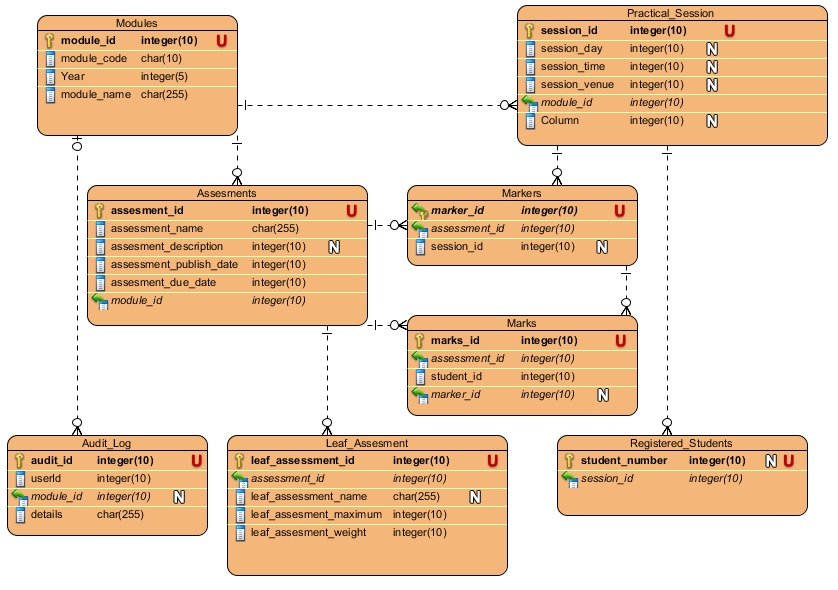
\includegraphics[scale=0.8]{./DatabaseDiagram/Backend_Database.jpg}
			2.1.1 The Database ERD Diagram\\\\
			\pagebreak
		\subsubsection{Back-end Class Diagram}
		The back end of Squirrel is the most important part. It handles all the business logic and database management. It will be implemented as a continuously running server awaiting connections from either the web interface or android application. It should be able to authenticate those connections, handle them and finally return the expected result. It should also update the audit trails accordingly. \\\\
			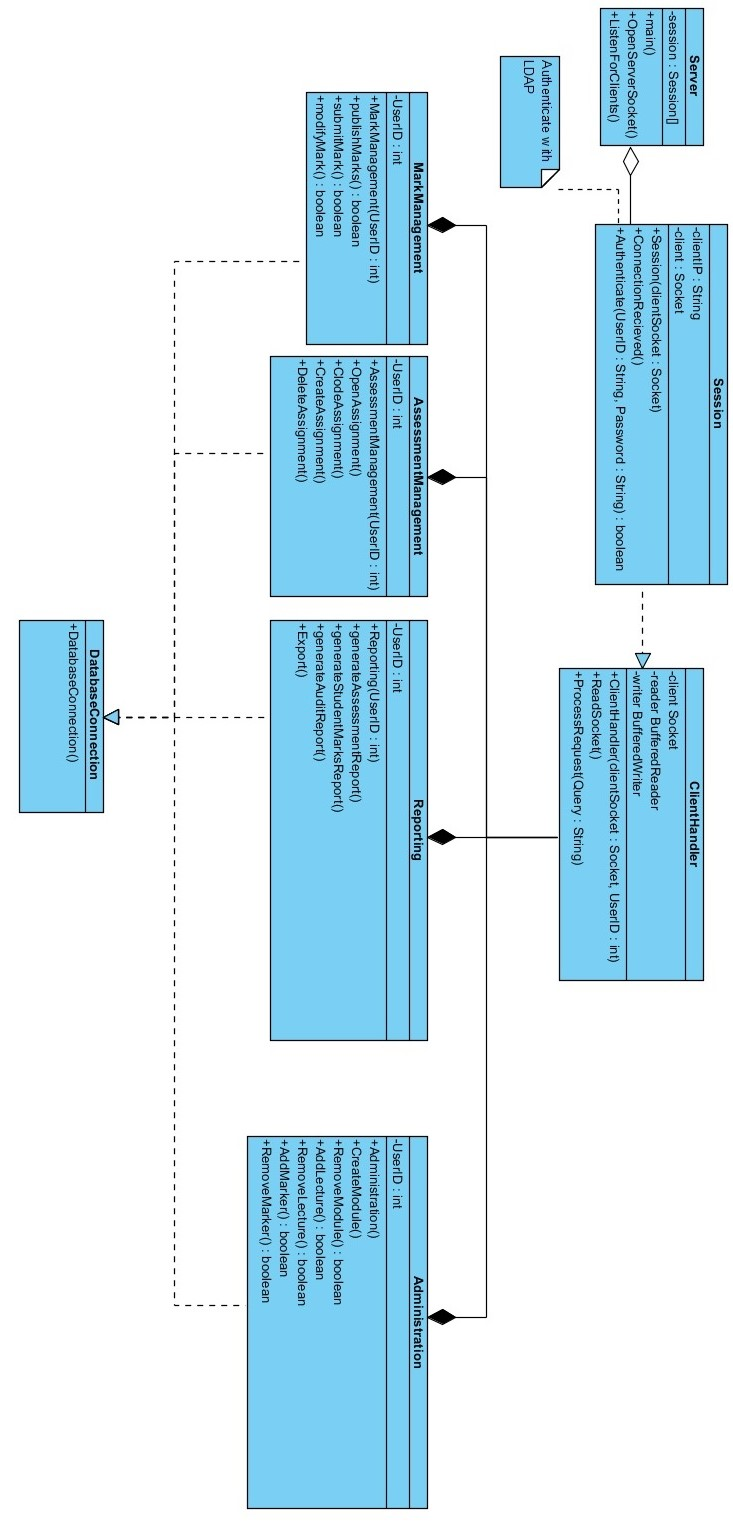
\includegraphics[scale=0.55]{./backendClasses.jpg}
			2.1.2 The Back-End Class Diagram\\\\
			\pagebreak
\subsection{Web Application}
The web application provides a browser based interface into our application as described in this section. The class diagram below provides the implementation-independent description of the types of processes that are used in the system and passed between its components. It conveys the input and output and possible exceptions that could occur within the application.\\\\
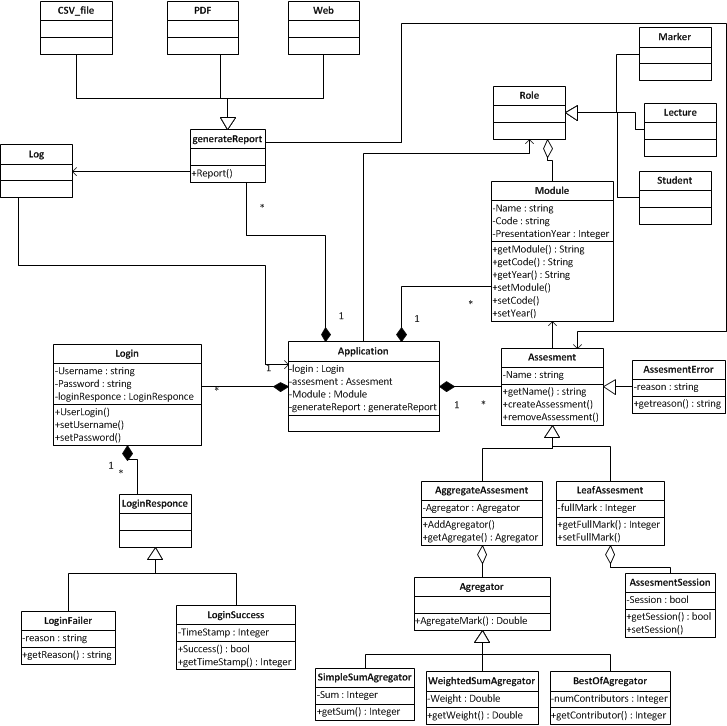
\includegraphics[scale = 0.75]{class_diagram.png}\\
2.2.1 The class Diagram of the web Application.\\\\
\textbf{Description of the class diagram}\\\\
The user provides his Login details and they are authenticated with the LDAP and if the details are incorrect an exception is thrown, else the user’s account is loaded to the application. Only the modules and assessment that the user is registered for can be viewed from the application. Through the application if the user is a student he can view his marks by generating a report. The lecture can create and maintain assessment by allocating student and markers to the leaf assessment and he is able of opening and closing an assessment as required. If a marker tries to modify or enter marks for an assessment session that he is not registered for, the application will throw an exception acknowledging the user of the error encountered.\\\\
The lecture can also maintain marks by allocating marks for student or editing marks and all of this a actions can take place while the assessment session of the mark sheet is open. The Lecture can generate an assessment report, student mark report and the audit log report when logged in as an administrator. When generating the report assessment or student mark report, the user can aggregate the marks by weight, and or by best of aggregate. The default aggregate is the sum aggregate and the reports can be generated as pdf, a CSV file or be displayed in the web application.\\\\
\textbf{The Activity Dargram}\\\\
Below is the activity diagram that describes the process specification of the web application

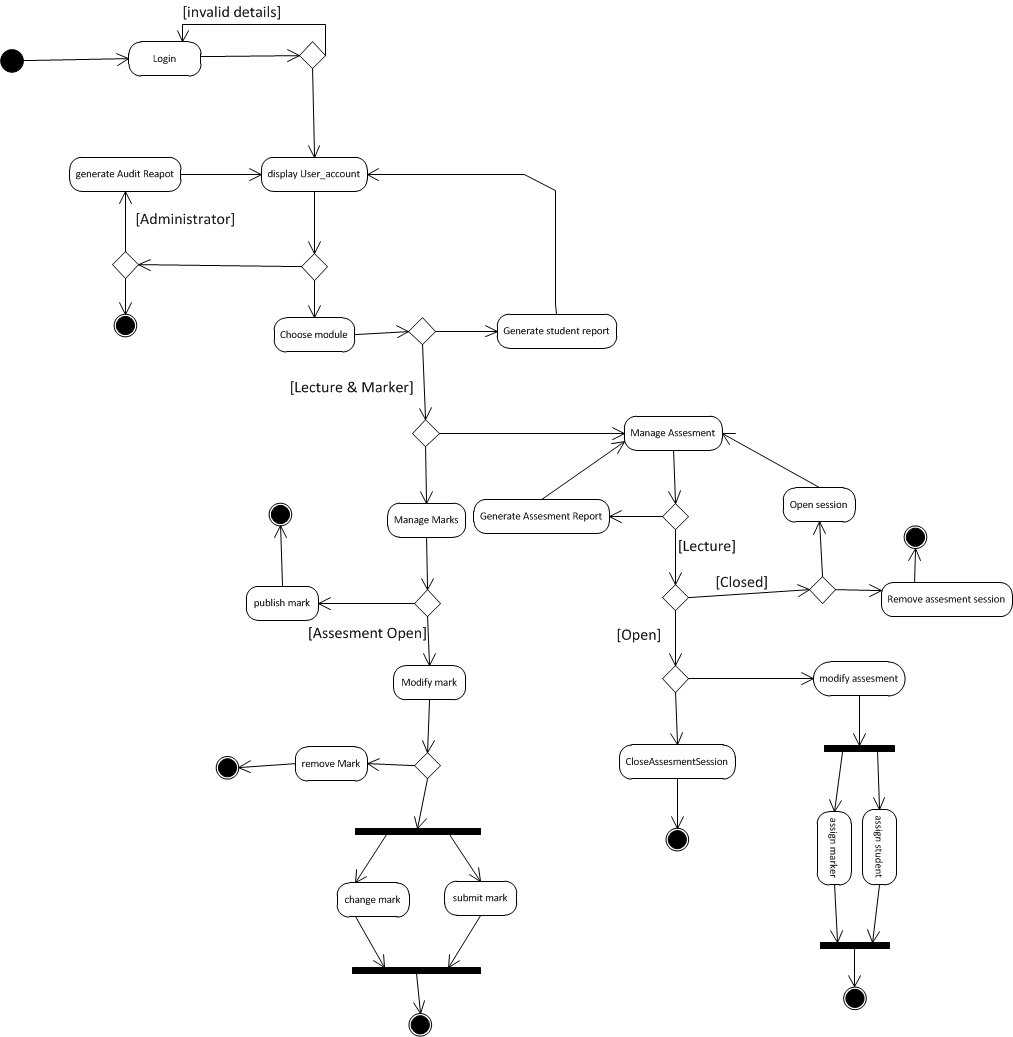
\includegraphics[scale=0.60]{activity_diagram.png}
2.2.2 The Activity diagram of the web Applictaion\\\\
\textbf{The process specification}\\\\
The user has to Login first in order to have access to the application, his details are authenticated and if details are invalid the user is returned to the application Login page, and an error displayed allowing the user to try inserting the correct details. If the login details are correct the home page is displayed with all the modules and assessment that the user is registered for. If the user is registered as an administrator, he can monitor and generate an audit log report.\\\\
The user can generate a student mark report and if a user is a lecture, he can manage marks as well as manage assessment. When managing marks the user can remove mark sheet and or publish it and if the assessment session of the mark sheet is open the lecture or assigned marker can change and submit student marks. The lecture can also create, modify and remove assessment session. He is also able to associate an assessment session to a group of students and markers. The lecture is also responsible for opening and closing assessment sessions.
\subsection{Android Application}
\subsubsection{Detailed System process specification}
All users need to enter a username and password when first opening the application on their android device.  This is necessary, for we do not want just anyone to be able to access the features and information that only specific users should have access to.\\\\
\textbf {Login:}
\begin{figure}[h]
\begin{center}
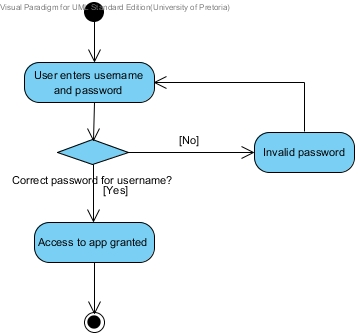
\includegraphics[scale=0.7]{./AndroidActivityDiagrams/ActivityDiagram1.jpg}
\end{center}
\end{figure}

After a user has gained access to the app, the user type (student/ teaching assistant/ lecturer) is detected.  The app only allows certain features to be available according to the user type\textquoteright s permissions.
\\

A student only has access to their own marks, thus when they choose to view marks, only their marks for the selected module are loaded. \\
\\
\textbf {Student views mark:}
\begin{figure}[h]
\begin{center}
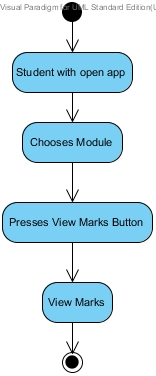
\includegraphics[scale=0.8]{./AndroidActivityDiagrams/ActivityDiagram2}
\end{center}
\end{figure} 

Students, like all users are however allowed to view the statistics for the selected module. \\
\\
\textbf {View statistics:}
\begin{figure}[h]
\begin{center}
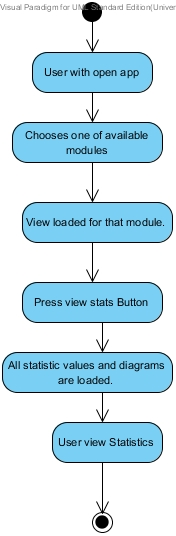
\includegraphics[scale=0.7]{./AndroidActivityDiagrams/ActivityDiagram3}
\end{center}
\end{figure}  

\newpage
\newpage
Both lecturers and TA’s should have the option to add marks for a student during the required specified time limit.\\
\\
\textbf {Adding marks:}
\begin{figure}[h]
\begin{center}
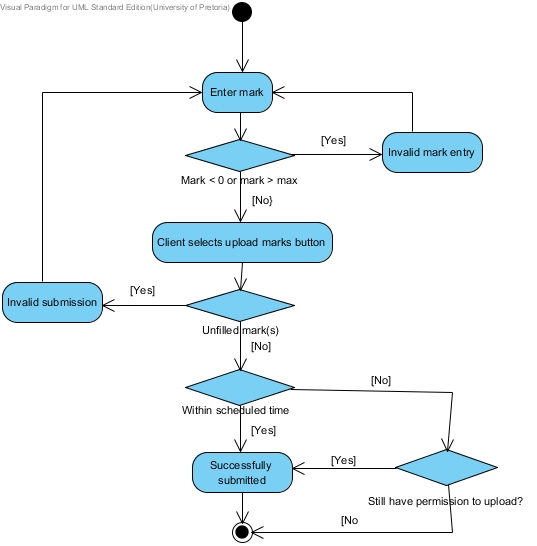
\includegraphics[scale=0.7]{./AndroidActivityDiagrams/ActivityDiagram5}
\end{center}
\end{figure}

\newpage
Only lecturers for a specific module should be able to edit marks after it has been uploaded.  Teaching will first need the permissions from the lecturer to be able to edit any marks.\\
\\
\textbf {Edit marks:}
\begin{figure}[h]
\begin{center}
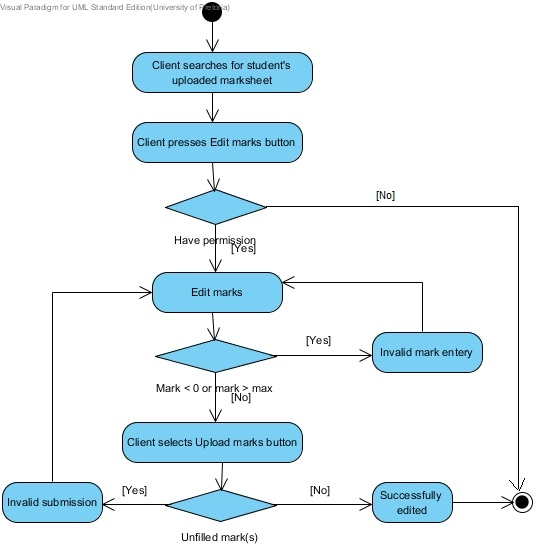
\includegraphics[scale=0.7]{./AndroidActivityDiagrams/ActivityDiagram6}
\end{center}
\end{figure}

\newpage
Only lecturers should be able to view all of the student's marks and give teaching assistants certain permissions.\\
\\
\textbf {Permissions and view all marks:}
\begin{figure}[h]
\begin{center}
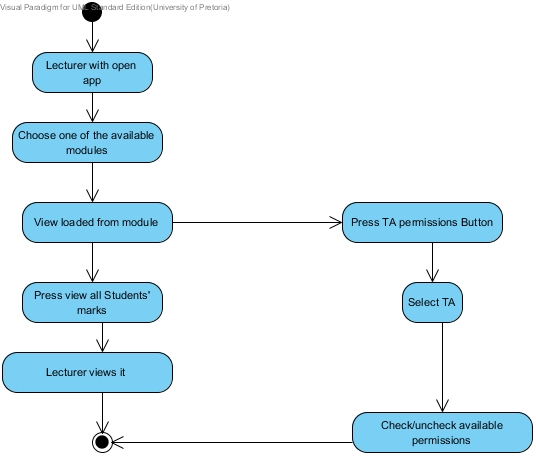
\includegraphics[scale=0.7]{./AndroidActivityDiagrams/ActivityDiagram4}
\end{center}
\end{figure}
\end{document}